\chapter{Integration Tests}

\section{CDU and Sensor}
\subsection{Integration test case 1: Sensor getinfo request}
\textbf{Purpose:}\\
The purpose of the test is to test the communication from CDU to Sensor node.\\

\textbf{Test equipment:}
\begin{itemize}
\item Analog Discovery USB oscilloscope
\item MPLAB X IDE
\item Explorer 16 board
\item ICD 3 Debugger
\item CDU stub
\item Sensor node with address 1
\end{itemize}

\textbf{Procedure:}\\
Apply 20 V on the P+ and P- pins of the CDU. Connect a sensor node to B+ and B- pins of the CDU. Connect the Explorer 16 board to the CDU circuit. Using the ICD 3 debugger, send a full message containing start sequence, address: "1" and function code: "1". Record what have been received on the sensor node circuit.\\

\textbf{Expected Result:}\\
A full message with address: "1" and function code: "1" has been received on the sensor node circuit.\\

\textbf{Actual Result:}\\
\begin{table}[H]
\centering
\begin{tabular}{|p{2cm}|p{2cm}|p{3cm}|p{2cm}|}\hline
\textbf{Test case:} & \textbf{Date:} & \textbf{Measurement:} & \textbf{Result:} \\ \hline
1 & 11-05-2014 & See below & PASSED \\ \hline
\end{tabular}
\end{table}
As seen below a full message with address: "1" and function code: "1" has been received.
\begin{figure}[H]
\centering
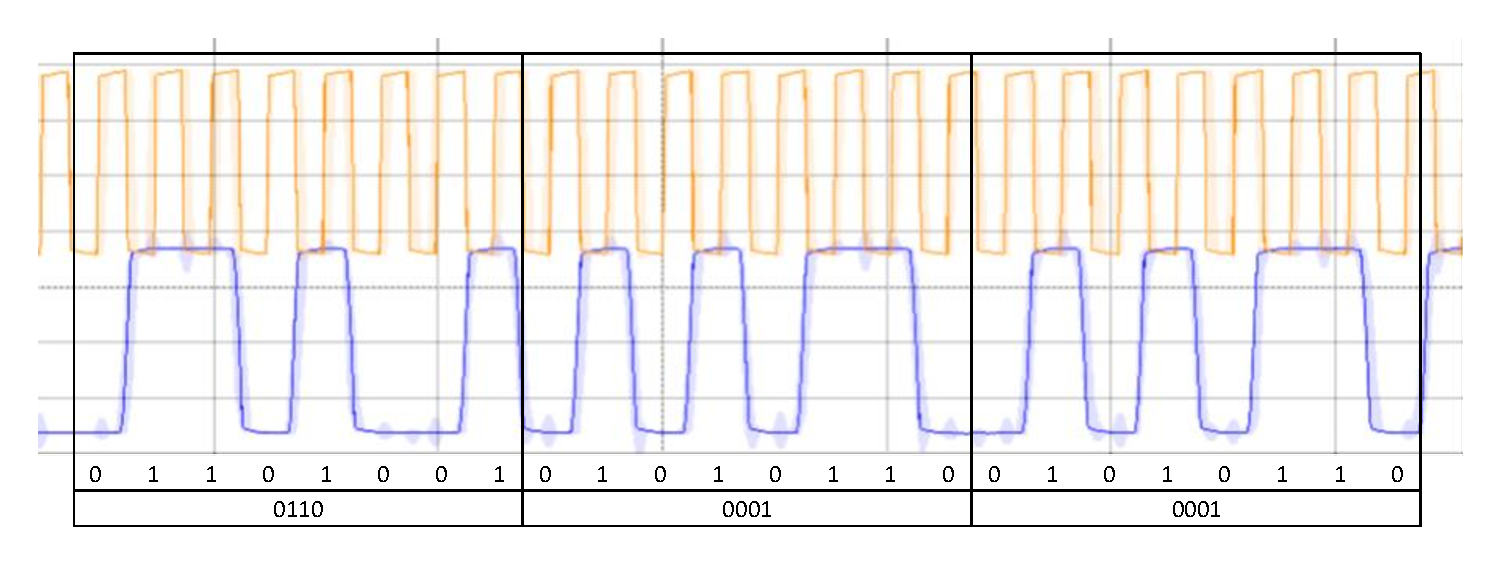
\includegraphics[width=0.8\textwidth]{billeder/CDUtestcase9}
\caption{Test Case 1 Result}
\label{fig:InteTestCase1}
\end{figure}

\textbf{Comment and remarks:}\\
-\\

\subsection{Integration test case 2: Sensor getdata request}
\textbf{Purpose:}\\
The purpose of the test is to test the communication from CDU to Sensor node.\\

\textbf{Test equipment:}
\begin{itemize}
\item Analog Discovery USB oscilloscope
\item MPLAB X IDE
\item Explorer 16 board
\item ICD 3 Debugger
\item CDU stub
\item Sensor node with address 1
\end{itemize}

\textbf{Procedure:}\\
Apply 20 V on the P+ and P- pins of the CDU. Connect a sensor node to B+ and B- pins of the CDU. Connect the Explorer 16 board to the CDU circuit. Using the ICD 3 debugger, send a full message containing start sequence, address: "1" and function code: "2". Record what have been received on the sensor node circuit.\\

\textbf{Expected Result:}\\
A full message with address: "1" and function code: "2" has been received on the sensor node circuit.\\

\textbf{Actual Result:}\\
\begin{table}[H]
\centering
\begin{tabular}{|p{2cm}|p{2cm}|p{3cm}|p{2cm}|}\hline
\textbf{Test case:} & \textbf{Date:} & \textbf{Measurement:} & \textbf{Result:} \\ \hline
2 & 15-05-2014 & See below & PASSED \\ \hline
\end{tabular}
\end{table}

\begin{figure}[H]
\centering
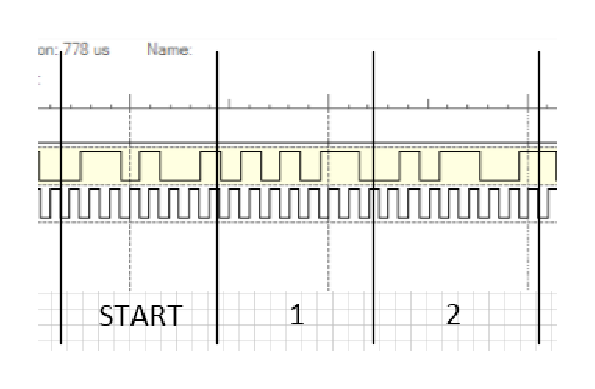
\includegraphics[width=0.8\textwidth]{billeder/intetestcase2}
\caption{Test Case 2 Result}
\label{fig:InteTestCase2}
\end{figure}

\textbf{Comment and remarks:}\\
-\\

\subsection{Integration test case 3: Sensor respond to getinfo}
\textbf{Purpose:}\\
The purpose of the test is to test the communication from a sensor node to the CDU.\\

\textbf{Test equipment:}
\begin{itemize}
\item Analog Discovery USB oscilloscope
\item MPLAB X IDE
\item Explorer 16 board
\item ICD 3 Debugger
\item CDU stub
\item Sensor node with address 1
\end{itemize}

\textbf{Procedure:}\\
Apply 20 V on the P+ and P- pins of the CDU. Connect a sensor node to B+ and B- pins of the CDU. Connect the Explorer 16 board to the CDU circuit. Using the sensor node logic and the CDU clock, send the getinfo response. Record what have been received on the CDU.

\textbf{Expected Result:}\\
A message containing address: "1", function code: "1" and the remainder of the response has been received.\\

\textbf{Actual Result:}\\
\begin{table}[H]
\centering
\begin{tabular}{|p{2cm}|p{2cm}|p{3cm}|p{2cm}|}\hline
\textbf{Test case:} & \textbf{Date:} & \textbf{Measurement:} & \textbf{Result:} \\ \hline
3 & - & - & - \\ \hline
\end{tabular}
\end{table}


\textbf{Comment and remarks:}\\
-\\

\subsection{Integration test case 4: Sensor respond to getdata}
\textbf{Purpose:}\\
The purpose of the test is to test the communication from a sensor node to the CDU.\\

\textbf{Test equipment:}
\begin{itemize}
\item Analog Discovery USB oscilloscope
\item MPLAB X IDE
\item Explorer 16 board
\item ICD 3 Debugger
\item CDU stub
\item Sensor node with address 1
\end{itemize}

\textbf{Procedure:}\\
Apply 20 V on the P+ and P- pins of the CDU. Connect a sensor node to B+ and B- pins of the CDU. Connect the Explorer 16 board to the CDU circuit. Using the sensor node logic and the CDU clock, send the getdata response. Record what have been received on the CDU.

\textbf{Expected Result:}\\
A message containing address: "1", function code: "2" and the remainder of the response has been received.\\

\textbf{Actual Result:}\\
\begin{table}[H]
\centering
\begin{tabular}{|p{2cm}|p{2cm}|p{3cm}|p{2cm}|}\hline
\textbf{Test case:} & \textbf{Date:} & \textbf{Measurement:} & \textbf{Result:} \\ \hline
4 & 15-05-2014 & See below & PASSED \\ \hline
\end{tabular}
\end{table}

\begin{figure}[H]
\centering
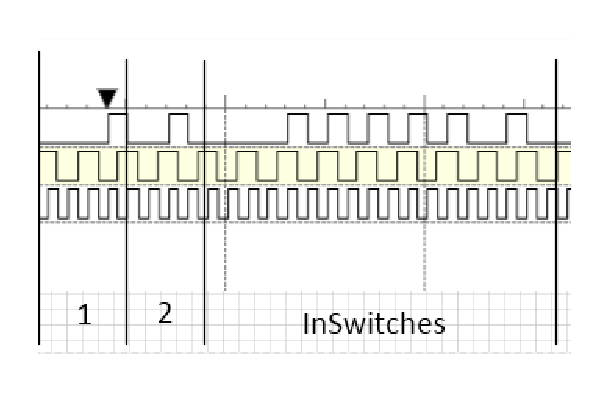
\includegraphics[width=0.8\textwidth]{billeder/intetestcase4}
\caption{Test Case 4 Result}
\label{fig:InteTestCase4}
\end{figure}


\textbf{Comment and remarks:}\\
-\\
\subsection{Integration test case 5: Full transmission}
\textbf{Purpose:}\\
The purpose of the test is to test the communication from the CDU to a sensor node and the response from the sensor node to the CDU.\\

\textbf{Test equipment:}
\begin{itemize}
\item Analog Discovery USB oscilloscope
\item MPLAB X IDE
\item Explorer 16 board
\item ICD 3 Debugger
\item CDU stub
\item Sensor node with address 1
\end{itemize}

\textbf{Procedure:}\\
Apply 20 V on the P+ and P- pins of the CDU. Connect a sensor node to B+ and B- pins of the CDU. Connect the Explorer 16 board to the CDU circuit. Using the ICD 3 debugger, send a full message containing start sequence, address: "1" and function code: "2". Record what have been received on CDU.\\

\textbf{Expected Result:}\\
A full response with address: "1" and function code: "2" has been received on the CDU. Data matches In-switches.\\

\textbf{Actual Result:}\\
\begin{table}[H]
\centering
\begin{tabular}{|p{2cm}|p{2cm}|p{3cm}|p{2cm}|}\hline
\textbf{Test case:} & \textbf{Date:} & \textbf{Measurement:} & \textbf{Result:} \\ \hline
5 & 15-05-2014 & See below & PASSED \\ \hline
\end{tabular}
\end{table}

\begin{figure}[H]
\centering
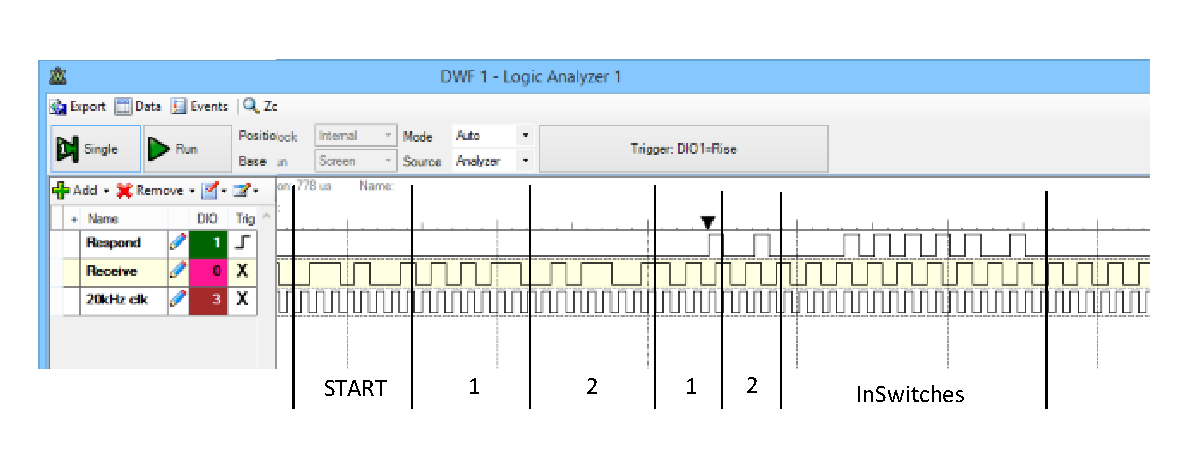
\includegraphics[width=0.8\textwidth]{billeder/intetestcase5}
\caption{Test Case 5 Result}
\label{fig:InteTestCase5}
\end{figure}


\textbf{Comment and remarks:}\\
-\\

\subsection{Integration test case 6: Full transmission, unknown function code}
\textbf{Purpose:}\\
The purpose of the test is to test the communication from the CDU to a sensor node and the response from the sensor node to the CDU.\\

\textbf{Test equipment:}
\begin{itemize}
\item Analog Discovery USB oscilloscope
\item MPLAB X IDE
\item Explorer 16 board
\item ICD 3 Debugger
\item CDU stub
\item Sensor node with address 1
\end{itemize}

\textbf{Procedure:}\\
Apply 20 V on the P+ and P- pins of the CDU. Connect a sensor node to B+ and B- pins of the CDU. Connect the Explorer 16 board to the CDU circuit. Using the ICD 3 debugger, send a full message containing start sequence, address: "1" and function code: "3". Record what have been received on the CDU.\\

\textbf{Expected Result:}\\
A full response with address: "1" and function code: "3" has been received on the CDU. Error code 2 is contained in the message.\\

\textbf{Actual Result:}\\
\begin{table}[H]
\centering
\begin{tabular}{|p{2cm}|p{2cm}|p{3cm}|p{2cm}|}\hline
\textbf{Test case:} & \textbf{Date:} & \textbf{Measurement:} & \textbf{Result:} \\ \hline
6 & - & - & - \\ \hline
\end{tabular}
\end{table}


\textbf{Comment and remarks:}\\
-\\


\section{CDU and PC}
\subsection{Integration test case 7: PC sends getdata request to CDU}
\textbf{Purpose:}\\
The purpose of the test is to test the communication from PC to the CDU.\\

\textbf{Test equipment:}
\begin{itemize}
\item Analog Discovery USB oscilloscope
\item MPLAB X IDE
\item Explorer 16 board
\item ICD 3 Debugger
\item CDU stub
\item Sensor node with address 1
\item Realterm software
\end{itemize}

\textbf{Procedure:}\\
Apply 20 V on the P+ and P- pins of the CDU. Connect a sensor node to B+ and B- pins of the CDU. Connect the Explorer 16 board to the CDU circuit. Connect the null modem cable to the Explorer 16 board and the PC. Open Realterm with the following settings: "38400 baud, 8 data bits, 1 stop bit and no parity". Press the RA7 button on the Explorer 16 Board. Send 'A' as ASCII from Realterm and observe the response. Load the data into a file.\\

\textbf{Expected Result:}\\
The memory printed in the RealTerm Terminal. The data is also logged to a file.\\

\textbf{Actual Result:}\\
\begin{table}[H]
\centering
\begin{tabular}{|p{2cm}|p{2cm}|p{3cm}|p{2cm}|}\hline
\textbf{Test case:} & \textbf{Date:} & \textbf{Measurement:} & \textbf{Result:} \\ \hline
7 & 12-05-2014 & See below & PASSED \\ \hline
\end{tabular}
\end{table}
Memory was printed to file. The data coincides with expected result.
\begin{figure}[H]
\centering
\includegraphics[width=1\textwidth]{billeder/inte07}
\caption{Test Case 7 Result}
\label{fig:InteTestCase7}
\end{figure}

\textbf{Comment and remarks:}\\
-\\

\subsection{Integration test case 8: PC sends unknown request to CDU}
\textbf{Purpose:}\\
The purpose of the test is to test the communication from PC to the CDU.\\

\textbf{Test equipment:}
\begin{itemize}
\item Analog Discovery USB oscilloscope
\item MPLAB X IDE
\item Explorer 16 board
\item ICD 3 Debugger
\item CDU stub
\item Sensor node with address 1
\end{itemize}

\textbf{Procedure:}\\
Apply 20 V on the P+ and P- pins of the CDU. Connect a sensor node to B+ and B- pins of the CDU. Connect the Explorer 16 board to the CDU circuit. Connect the null modem cable to the Explorer 16 board and the PC. Open Realterm with the following settings: "38400 baud, 8 data bits, 1 stop bit and no parity". Press the RA7 button on the Explorer 16 Board. Send 'U' as ASCII from Realterm and observe the response.\\

\textbf{Expected Result:}\\
unknown cmd is printed to the terminal.\\

\textbf{Actual Result:}\\
\begin{table}[H]
\centering
\begin{tabular}{|p{2cm}|p{2cm}|p{3cm}|p{2cm}|}\hline
\textbf{Test case:} & \textbf{Date:} & \textbf{Measurement:} & \textbf{Result:} \\ \hline
8 & 12-05-2014 & See below & PASSED \\ \hline
\end{tabular}
\end{table}
unknown cmd was printed to the terminal as shown on figure ~\ref{fig:InteTestCase8}.
\begin{figure}[H]
\centering
\includegraphics[width=1\textwidth]{billeder/inte08}
\caption{Test Case 8 Result}
\label{fig:InteTestCase8}
\end{figure}

\textbf{Comment and remarks:}\\
-\\